\documentclass[tikz]{standalone}
\usetikzlibrary{calc,angles,quotes}
\begin{document}
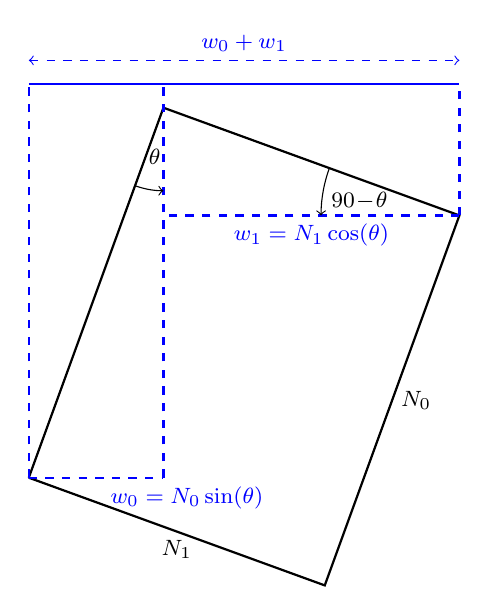
\begin{tikzpicture}[scale=2]
  \footnotesize

  % Define rectangle dimensions
  \def\width{2}       % base width
  \def\aspect{1.25}   % aspect ratio (height/width)
  \pgfmathsetmacro{\height}{\width*\aspect}

  % Rotate rectangle by 20 degrees
  \begin{scope}[rotate around={-20:(0,0)}]
    % Draw rectangle with bottom-left corner at origin
    \draw[thick] (0,0) -| (\width,\height)
           node[pos=0.25,below] {$N_1$}
           node[pos=0.75,right] {$N_0$}
           -| (0,0);

    % Save post-rotation rectangle corners
    \coordinate (BL) at (0,0);
    \coordinate (BR) at (\width,0);
    \coordinate (TL) at (0,\height);
    \coordinate (TR) at (\width,\height);
  \end{scope}

  \def\liney{2.5} % top line height
  \coordinate (PL) at (BL |- 0,\liney); % vertical intersection from bottom-left
  \coordinate (PR) at (TR |- 0,\liney); % vertical intersection from top-right

   % Horizontal line representing sensor
  \draw[blue,thick] (PL) -- (PR);

  % Draw verticals to meet horizontal line
  \draw[blue,thick,dashed] (BL) -- (PL);
  \draw[blue,thick,dashed] (TR) -- (PR);

  % Double-sided arrow for width label
  \draw[<->,blue,dashed] (PL) ++(0,0.15) -- ($(PR)+(0,0.15)$)
    node[midway,above] {$w_0 + w_1$};

  % Central vertical line through top-left corner
  \draw[blue,thick,dashed] (TL |- BL) -- (TL |- 0,\liney);

  % Horizontal lines with labels
  \draw[blue,thick,dashed] (TR) -- (TL |- TR) node[midway,below] {$w_1 = N_1 \cos(\theta)$};
  \draw[blue,thick,dashed] (BL) -- (TL |- BL) node[right,below] {$\qquad w_0 = N_0 \sin(\theta)$};

  % Define intersection point with central vertical line
  \coordinate (VL) at (TL |- BR);
  \coordinate (HL) at (TL |- TR);

  % θ between left rectangle side and central vertical line
  \pic [draw, ->, "$\theta$", angle radius=30] {angle = BL--TL--VL};

  % 90-θ between top rectangle side and horizontal line
  \pic [draw, ->, "$90\!-\!\theta\quad\;\;$", angle radius=50] {angle = TL--TR--HL};

\end{tikzpicture}
\end{document}
